\chapter{Mod\`ele de donn\'ees}
	La base de donn\'ees est l'une des parties du \textit{3-tier architecture} que nous avons choisi d'adopter (Voir chapitre~\ref{ChapArchitectureDuSysteme}). Pour satisfaire aux besoins du syst\`eme elle doit fournir un moyen efficace et s\'ecuris\'e du g\'erer les donn\'ees et autres formes d'informations du syst\`eme et doit disposer des points d'entr\'es n\'ecessaire pour une communication efficace avec le serveur d'application. En fin, tout cela doit imp\'erativement se faire de fa\c{c}on s\'ecuris\'ee.

	\paragraph{} Un mod\`ele de donn\'ees permet de d\'ecrire des donn\'ees ou des informations\cite{ModeleDeDonneesDefinition} en d\'efinissant leur structure, les contraintes auxquelle elles sont soumises ainsi que les op\'eration qui peuvent \^etre effectu\'ees sur elles. C'est un outil incontournable pour la conception, la mise en \oe{}uvre et la maintenance d'une base de donn\'ees.


	\paragraph{} Lors de la conception, le mod\`ele permet de garantir la coh\'erence et l'int\'egrit\'e dans la base de donn\'ees tout en am\'eliorant sa performance. Plus tard, il va garantir que les donn\'ees pourront \^etre trait\'ees sans erreurs (exactitude des donn\'ees), que la base de donn\'ees pourra maintenir ses fonctionnalit\'es et sa performance face \`a une grande augmentation/diminution du nombre d'utilisateurs (extensibilit\'e de la BDD). De plus, la documentation claire que fournit le mod\`ele va faciliter la maintenance et l'\'evolution la base de donn\'ees car cette documentation permet de bien identifier les impacts que  des changements peuvent avoir sur la base de donn\'ees.

	\paragraph{} Il existe plusieurs mod\`eles comme le mod\`ele semi-structur\'e, le mod\`ele hi'erarchique, le mod\`ele relationnel, le mod\'ele entit\'e-association\cite{ModeleDeDonneesDefinition}, etc. Dans notre cas, nous avons choisi le mod\`ele relationnel parce qu'il est simple \`a concevoir, \`a maintenir et \`a utiliser. De plus le mod\`ele relationnel offre la possibilit\'e d'utiliser un langage de requ\^ete, comme SQL, pour g\'en\'erer des informations \`a partir des donn\'ees stock\'ees dans la BDD. Cette fonctionnalit\'ee sera tr\`es exploit\'ee dans notre travail.




	\section{Structure de donn\'ees dans la base}
		\paragraph{} \textbf{Pour d\'eterminer la structure des donn\'ees, nous allons proc\'eder aux \'etapes suivantes :}

		\begin{enumerate}
			\item[1] Pr\'esenter les objectifs g\'en\'erales de la base de donn\'ees
			\item[2] Identifier les concepts pr\'esents dans les donn\'ees que va g\'erer le projet.
			\item[3] Organisation des donn\'ees en relations et sp\'ecification des cl\'es primaires
			\item[4] Normalisation des relations
			\begin{itemize}
				\item[4.1] Normalisation suivant la $1^{ere}$ forme normale
				\item[4.2] Normalisation suivant la $2^{eme}$ forme normale
				\item[4.3] Normalisation suivant la $3^{eme}$ forme normale
			\end{itemize}
			\item[5] Analyser liens entre les relations et sp\'ecificier des cl\'es \'etrang\`eres
			\item[6] \'Elaborer un dictionnaire de donn\'ees
		\end{enumerate}
		\vspace{1cm}



		\subsection{Objectifs de la base de donn\'ees}
			\begin{itemize}
				\item[\_] Nous voulons construire une base de donn\'ees pour entreposer des documents, des images, des vid\'eos et des contenus audio.
				\item[\_] L'ensemble des ressources de la base doit \^etre accessibles via Internet pour \^etre consult\'es, t\'el\'echarg\'es ou partag\'es par les utilisateurs.
				\item[\_] Ces contenus seront regroup\'es en cat\'egories.
				\item[\_] Il ne sera pas n\'ecessaire de garder des informations d\'etaill\'ees sur les utilisateurs.
				\item[\_] Tous utilisateur peut laisser une note \`a chaque ressources qu'il a consult\'e.
				\item[\_] Les administrateurs doivent pouvoir g\'erer la base de donn\'ees
			\end{itemize}



		\subsection{Les concepts}
			Les principaux concepts qui reviennent dans la sp\'ecification des objectifs de la base de donn\'ees sont les suivants :
			\begin{itemize}
				\item[-] Document
				\item[-] Cat\'egorie
				\item[-] Administrateur
				\item[-] utilisateur
			\end{itemize}



		\subsection{Organisation des donn\'ees en relations et sp\'ecification des cl\'es primaires}
			Dans le mod\`ele de relationnel, nous devons cr\'eer une relation pour stocker les donn\'ees concernant chacun de ces concepts.

			\paragraph{}Nous cr\'eons donc les relations suivantes :

				\subsubsection{Documents}
				\label{SectionRelationDocuments}
					Dans cette relation nous stockons tous ce qui a rapport avec les contenus auxquels le syst\`eme permettra l'acc\`es. La relation Documents contient les champs suivants :\\


				\begin{tabularx}{500pt}{>{- }m{4cm} X} %{>{\hsize=.5\hsize\linewidth=\hsize}X >{\hsize=.5\hsize\linewidth=\hsize}X}

					%\textit{idDocument \newline(Cl\'e primaire)} & Code permettant d'identifier un document de fa\c{c}on unique dans la BDD.\\

					\textit{Titre} & Couramment appel\'e « Nom » d'un document. C'est une cha\^ine de caract\`eres qui permettra de reconna\^itre le document lors qu'on utilise la plateforme. \\

					\textit{Resume} & Il s'agit d'un court r\'esum\'e qui permet de conna\^itre les diff\'erents th\`emes et sujets qui sont trait\'es dans le document.\\

					\textit{Taille} & C'est le nombre des bytes qui constitue le fichier document.\\

					\textit{Fichier} & Lien vers le fichier correspondant au document dans le syst\`eme de fichiers. \\

					\textit{NombreDeConsultations} & Nombre de fois qu'un utilisateur a consult\'e un document depuis que ce dernier a \'et\'e mis en ligne.\\

					\textit{NombreDePartages} & Nombre de fois qu'un utilisateur a partag\'e un document depuis que ce dernier a \'et\'e mis en ligne.\\

					\textit{TypeDeFichier} & Pr\'ecise si le fichier est une image, une vid\'eo, un document textuel ou un fichier audio.\\

					\textit{Langue} & Langue du contenu. \\

					\textit{Note} & Moyenne des notes que les utilisateurs ont donn\'e \`a un document.\\

					\textit{NombreDeNote} & Nombre de fois qu'un utilisateur a not\'e ce document depuis que ce dernier a \'et\'e mis en ligne. \\

					\textit{Etiquette} & Ensemble de termes auxquels le document est rattach\'e. Les \'etiquettes facilitent la recherche dans la base de donn\'ees. \\

					\textit{Auteur} & Personnes (physique) ayant droit d'auteur sur ce document.\\

					\textit{DateCreationDocument} & Date \`a laquelle le document a \'et\'e enregistr\'e dans la base de donn\'ees. \\

					\textit{AuteurCreationDocument} & Utilisateur ayant enregistr\'e le document dans la base de donn\'ees (Nom et pr\'enom concaten\'es).\\

					\textit{DateModificationDocument} & Date \`a laquelle le document a \'et\'e modifi\'e pour la derni\`ere fois dans la base de donn\'ees. \\

					\textit{AuteurModificationDocument} & Utilisateur ayant effectu\'e la derni\`ere modification sur le document (Nom et pr\'enom concaten\'es).\\

					\textit{SupprimerDocument} & Dit si l'enregistrement doit \^etre affich\'e sur le site ou non. \\


				\end{tabularx}

				\subsubsection*{Categories}

					\begin{tabularx}{500pt}{>{- }m{4cm} X}
						\textit{IdCategorie \newline(Cl\'e primaire)} & Code permettant d'identifier une cat\'egorie de fa\c{c}on unique dans la BDD.\\

						\textit{NomCategorie} & Cha\^ine de caract\`eres qui permettra de reconna\^itre une cat\'egorie. \\

						\textit{DateCreationCategorie} & Date \`a laquelle la cat\'egorie a \'et\'e cr\'e\'ee dans la base de donn\'ees. \\

						\textit{AuteurCreationCategorie} & Utilisateur ayant cr\'e\'e la cat\'egorie dans la base de donn\'ees (Nom et pr\'enom concat\'es).\\

						\textit{DateModificationCategorie} & Date \`a laquelle la cat\'egorie a \'et\'e modifi\'ee pour la derni\`ere fois dans la base de donn\'ees. \\

						\textit{AuteurModificationCategorie} & Utilisateur ayant effectu\'e la derni\`ere modification sur la cat\'egorie (Nom et pr\'enom concat\'es). \\

						\textit{SupprimerCategorie} & Dit si l'enregistrement doit \^etre affich\'e et utilis\'e sur le site ou non. \\
					\end{tabularx}

				\vspace{1cm}


				% (Nom et pr\'enom concat\'es) fòk mw korije l pou m met konkatENe
				\subsection*{Utilisateurs}

					\begin{tabularx}{500pt}{>{- }m{4cm} X}
						\textit{IdUtil \newline(Cl\'e primaire)} & Code permettant d'identifier un utilisateur de fa\c{c}on unique dans la BDD. \\

						\textit{NomUtil} & Nom de famille de l'utilisateur.\\

						\textit{PrenomUtil} & Pr\'enom de l'utilisateur. \\

						\textit{E-mailUtil} & Adresse \'electronique de l'utilisateur. \\

						\textit{MotDePasseUtil} & Mot de passe de l'utilisateur. \\

						\textit{Administrateur} & Permet de savoir si cette utilisateur poss\`ede les droits d'un administrateur.\\

						\textit{DateCreationUtil} & Date \`a laquelle l'utilisateur a \'et\'e cr\'e\'e dans la base de donn\'ees.\\

						\textit{AuteurCreationUtil} & Utilisateur ayant cr\'e\'e l'utilisateur dans la base de donn\'ees (Nom et pr\'enom concaten\'es).\\

						\textit{DateModificationUtil} & Date \`a laquelle l'utilisateur a \'et\'e modifi\'ee pour la derni\`ere fois dans la base de donn\'ees. \\

						\textit{AuteurModificationUtil} & Utilisateur ayant effectu\'e la derni\`ere modification sur l'enregistrement (Nom et pr\'enom concaten\'es).\\

						\textit{SupprimerUtil} & Dit si l'enregistrement doit \^etre affich\'e et utilis\'e sur le site ou non. \\

					\end{tabularx}




		\subsection{Normalisation des relations}
			Pour concevoir un mod\`ele donn\'ees relationnel correct, les relations doivent respecter un ensemble de r\`egles appel\'ees les formes normales. Pour cela nous allons v\'erifier que nos relations respectent les trois premi\`eres formes normales.\\


			\subsubsection{1$^{ere}$ forme normale} Cette condition exige que tous les champs d'une relation soient atomiques. En d'autres termes, chaque champ ne doit contenir qu'une seule information. Or, dans la relation des Documents, les champs Etiquette et Auteur peuvent avoir plusieurs valeurs. En effet un m\^eme document pourrait avoir plusieurs \'etiquettes ou plusieurs auteurs. Pour traiter ces cas, en plus de la table de base qui contient les donn\'ees des documents, nous cr\'eons des tables \`a part enti\`ere pour stocker les donn\'ees de chacun des champs en question. La relation Document sera une vue cr\'e\'ee \`a partir des tables ad\'equates. D'o\`u les  suivantes:



			\paragraph{} \textbf{Etiquette}

			\begin{tabularx}{500pt}{>{- }m{5cm} X}

				\textit{IdEtiquette \newline(Cl\'e primaire)} & Code permettant d'identifier un \'etiquette de fa\c{c}on unique dans la base de donn\'ees.\\

				\textit{Etiquette} & Cha\^ine de caract\`eres qui permettra de reconna\^itre un \'etiquette.\\

				\textit{DateCreationEtiquette} & Date \`a laquelle l'\'etiquette a \'et\'e cr\'e\'ee dans la base de donn\'ees.\\

				\textit{AuteurCreationEtiquette} & Utilisateur ayant cr\'e\'e l'\'etiquette dans la base de donn\'ees.\\

				\textit{DateModifEtiquette} & Date \`a laquelle l'\'etiquette a \'et\'e modifi\'ee pour la derni\`ere fois dans la base de donn\'ees.\\

				\textit{AuteurModifEtiquette} & Utilisateur ayant effectu\'e la derni\`ere modification sur l'\'etiquette. \\

				\textit{SupprimerEtiquette} & Dit si l'enregistrement doit \^etre affich\'e et utilis\'e sur le site ou non.  \\
			\end{tabularx}
			%\vspace{1cm}}

%				\newpage

			\paragraph{} \textbf{Auteur}

			\begin{tabularx}{500pt}{>{- }m{4cm} X}

				\textit{IdAuteur  \newline(Cl\'e primaire)} & Code permettant d'identifier un propri\'etaire de fa\c{c}on unique dans la base de donn\'ees. \\

				\textit{NomAuteur} & Nom de famille de l'auteur.\\

				\textit{PrenomAuteur} & Pr\'enom de l'auteur. \\

				\textit{EmailAuteur} & Adresse \'electronique de l'utilisateur. \\

				\textit{NationnaliteAuteur} & Nationnalit\'e de l'auteur.\\

				\textit{DateCreationAuteur} & Date \`a laquelle l'auteur a \'et\'e cr\'e\'ee dans la base de donn\'ees.\\

				\textit{AuteurCreationAuteur} & Utilisateur ayant cr\'e\'e l'enregistrement dans la base de donn\'ees.\\

				\textit{DateModifAuteur} & Date \`a laquelle l'enregistrement a \'et\'e modifi\'ee pour la derni\`ere fois dans la base de donn\'ees.\\

				\textit{AuteurModifAuteur} & Utilisateur ayant effectu\'e la derni\`ere modification sur l'enregistrement. \\

				\textit{SupprimerAuteur} & Dit si l'enregistrement doit \^etre affich\'e et utilis\'e sur le site ou non.  \\
			\end{tabularx}


			\subsubsection{2$^{eme}$ forme normale}
				La deuxi\`eme forme normale exige que chaque champ de la relation d\'epende enti\`erement de la cl\'e primaire.\\
				Tous les relations satisfont \`a cette exigence.

				\vspace{1cm}


			\subsubsection{3$^{eme}$ forme normale}
				Elle exige qu'aucun champ non-cl\'e ne d\'epende d'un autre attribut non-cl\'e.\\
				Les relations satisfont \`a cette exigence.

				\vspace{1cm}



		\subsection{Analyser les liens entre les relations}
			Les tables sont reli\'ees entre eux comme sur la figure~\ref{RelationEntreTables}.


			\begin{figure}[!ht]
				\centering
				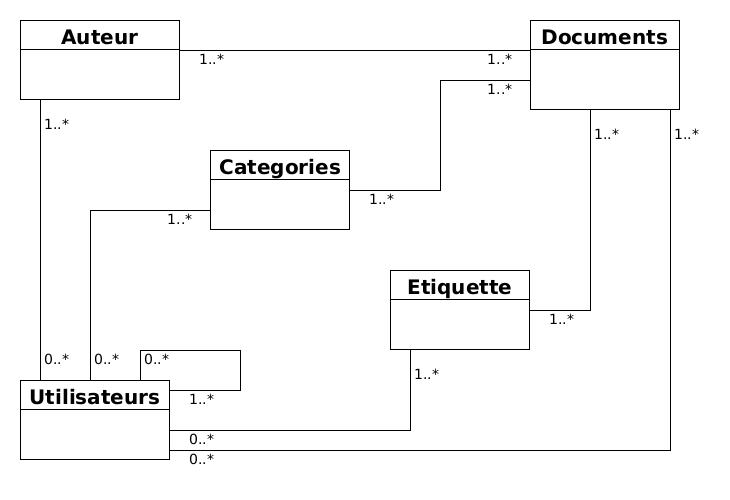
\includegraphics[width=0.75\linewidth]{Pictures/RelationEntreLesTables.jpg}
				\caption{Liens entre les relations}
				\label{RelationEntreTables}
			\end{figure}


			\paragraph{}Dans le mod\`ele de donn\'es relationnel, on cr\'ee un lien du type  plusieurs \`a plusieurs en ajoutant une nouvelle table qui recevra les cl\'es primaires des relations \`a relier comme cl\'es \'etrang\`eres. Par cons\'equent, chacun de ces liens va donner naissance \`a une nouvelle table. Ainsi, nous cr\'eerons huit nouvelles tables qui peuvent \^etre r\'eparties en deux groupes suivant les champs qui les composent:% Toutefois, \'etant donn\'e que tous , nous avons d\'ecid\'e de les unir en une seule relation nomm\'ee \textit{Gestion}. Pour les m\^emes raisons, les autres tables sont unies pour former la table tableRelation.

			\paragraph{}Nous obtenons ainsi les relations suivantes:


			\subsubsection*{Les tables de gestion}
				Les tables des liens entre la relation Utilisateur et les autres auront rigoureusement les m\^emes champs:

				\begin{tabularx}{500pt}{>{- }m{4cm} X}
					\textit{ IdentifiantAdmin \newline(Cl\'e \'etrang\`ere) \newline(Cl\'e primaire)} & Code permettant d'identifier l'administrateur qui a effectu\'e le changement. \\
					\textit{ IdentifiantXxxx \newline(Cl\'e \'etrang\`ere) \newline(Cl\'e primaire)} & Code permettant d'identifier l'\'el\'ement qui a subit le changement.  \\
					\textit{Date} & Date \`a laquelle le changement a \'et\'e effectu\'e. \\
					\textit{TypeGestion} & Pr\'ecise s'il s'agit d'un ajout, d'une suppression, ... \\
				\end{tabularx}
				\vspace{.5cm}


			\subsubsection*{Les tables de liaison}
				Les tables qui lient la table tableDocuments aux autres tables (Except\'e tableUtilisateurs) ont aussi les m\^emes champs: \\

				\begin{tabularx}{500pt}{>{- }m{4cm} X}

					\textit{ idDocument \newline(Cl\'e \'etrang\`ere) \newline(Cl\'e primaire)} & Code permettant d'identifier le document li\'e. \\

					\textit{ idXxxx \newline(Cl\'e \'etrang\`ere) \newline(Cl\'e primaire)} & Code permettant d'identifier un enregistrement dans une autre table auquel le document est li\'e.\\
				\end{tabularx}

			\subsubsection*{Autres tables}
				L'impl\'ementation de la fonction de recherche, telle que nous la concevons, requiert l'utilisation de deux autres tables.

				\paragraph{} \textbf{Stopwords}\\
				Pour stocker nos Stopwords\footnote{Fonctionnalit\'e de mariadb. Il s'agit d'une liste de mot qui seront ignor\'e lors des recherches pour cause qu'ils sont consid\'er\'e comme d\'enu\'e de sens propre (Voir \href{https://mariadb.com/kb/en/full-text-index-stopwords/}{Mariadb Stopwords})} personnalis\'es dans le serveur.

				\begin{tabularx}{500pt}{>{- }m{4cm} X}

					\textit{ idMot\_d\_arret \newline(Cl\'e primaire)} & Code permettant d'identifier chaque enregistrement de fa\c{c}on unique. \\

					\textit{ Mot\_d\_arret} & Stopword.\\
				\end{tabularx}


				\paragraph{} \textbf{Dictionnaire}\\
				Pour stocker tous les mots utilis\'es dans la base de donn\'ees \`a l'excetption des stopwords.

				\begin{tabularx}{550pt}{>{- }m{4cm} X}

					\textit{ idMot \newline(Cl\'e primaire)} & Code permettant d'identifier chaque enregistrement de fa\c{c}on unique. \\

					\textit{ Mot } & Mot utilis\'e dans la base de donn\'ees.\\
				\end{tabularx}



		\subsection{Dictionnaire de donn\'ees}
			Le tableau~\ref{DictionnaireDeDonnees} pr\'esente la liste des relations \`a cr\'eer pour constituer la base de donn\'ees.
			\vspace{1cm}


            \begin{center}
			\begin{longtable}[c]{| m{0.22\linewidth}  m{0.3\linewidth}  m{0.16\linewidth}  m{0.22\linewidth} |}
%				\centering
                \caption{Dictionnaire de donn\'ees.} \label{DictionnaireDeDonnees} \\

					\hline
					\hline
					\rowcolor{TetTablo}
                    \textbf{\textsc{\Large{Nom}}} & \textbf{\textsc{\Large{Code}}} & \textbf{\textsc{\Large{Type}}} & \textbf{\textsc{\Large{Note}}}\\
					\hline
					\hline
					\endfirsthead

					\hline
					\hline
					\rowcolor{TetTablo}
					\textbf{\textsc{\Large{Nom}}} & \textbf{\textsc{\Large{Code}}} & \textbf{\textsc{\Large{Type}}} & \textbf{\textsc{\Large{Note}}}\\
					\hline
					\hline
					\endhead

					\hline
					\endfoot

					\hline
					\hline
					\endlastfoot

					\rowcolor{mybrown}
					\multicolumn{4}{l}{tableDocuments}\\
					Identifiant & PK\_idDocument & INT & Non sign\'e, Non nul, Auto-incr\'ement\'e, cl\'e primaire\\
					Titre & TITRE & VARCHAR(255) & Non nul\\
					R\'esum\'e & RESUME & TEXT & \\
					Taille & TAILLE & INT & Non sign\'e\\
					Adresse du fichier & FICHIER & VARCHAR(255) & Non nul\\
					Nombre de consultation & NombreDeConsultations & DOUBLE & Non nul, Non sign\'e\\
					Nombre de partages  & NombreDePartages & DOUBLE & Non nul, Non sign\'e \\
					Type de fichier & TypeFichier & ENUM & Non nul\\
					Langue & LANGUE & ENUM & \\
					Note  & NOTE & FLOAT & Non sign\'e, Non nul\\
					Nombre de notes  & NombreNotes & DOUBLE & Non sign\'e, Non nul\\
					Cr\'eation & DateCreationDocument & DATE & Non nul\\
					Admin\_Cr\'eation & AuteurCreationDocument & VARCHAR(255) & Non nul\\
					Derni\`ere modification & DateModificationDocument & DATE & Non nul\\
					Admin\_Modification & AuteurModificationDocument & VARCHAR(255) & Non nul\\
					Supprim\'e & SupprimerDocument & BOOLEAN & Non nul\\

					\rowcolor{mybrown}
					\multicolumn{4}{l}{tableCategories} \\
					Identifiant & PK\_idCategorie & INT & Non sign\'e, Non nul, Auto-incr\'ement\'e, cl\'e primaire\\
					Cat\'egorie & CATEGORIE & VARCHAR(31) & Unique, Non nul\\
					Date de cr\'eation & DateCreationCategorie & DATE & Non nul\\
					Admin\_Cr\'eation & AuteurCreationCategorie & VARCHAR(255) & Non nul\\
					Date derni\`ere modification & DateModificationCategorie & DATE & Non nul\\
					Admin\_Modification & AuteurModificationCategorie & VARCHAR(255) & Non null\\
					Supprim\'e & SupprimerCategorie & BOOLEAN & Non nul\\

					\rowcolor{mybrown}
					\multicolumn{4}{l}{tableUtilisateurs} \\
					Identifiant & PK\_idUtil & INT & Non sign\'e, Non nul, Auto-incr\'ement\'e, cl\'e primaire\\
					Nom & NomUtil & VARCHAR(31) &  \\
					Pr\'enom  & PrenomUtil & VARCHAR(31) & \\
					Nom d'utilisateur  & USERNAME & VARCHAR(31) & Unique\\
					Addresse IP  & AddresseIP & VARCHAR(128) & \\
					E-mail & EmailUtil & VARCHAR(255) & \\
					Mot de passe & MotDePasseUtil & VARCHAR(255) & \\
					Administrateur & Administrateur & BOOLEAN & Non nul\\
					Date de cr\'eation & DateCreationUtil & DATE & Non nul\\
					Admin\_Cr\'eation & AuteurCreationUtil & VARCHAR(255) & Non nul\\
					Date derni\`ere modification & DateModificationUtil & DATE & Non nul\\
					Admin\_Modification & AuteurModificationUtil & VARCHAR(255) & Non nul\\
					Supprim\'e & SupprimerUtil & BOOLEAN & Non nul\\

					\rowcolor{mybrown}
					\multicolumn{4}{l}{tableEtiquettes} \\
					Identifiant & PK\_idEtiquette & INT & Non sign\'e, Non nul, Auto-incr\'ement\'e, cl\'e primaire\\
					\'Etiquette & ETIQUETTE & VARCHAR(31) & Unique, Non nul\\
					Date de cr\'eation & DateCreationEtiquette & DATE & Non nul\\
					Admin\_Cr\'eation & AuteurCreationEtiquette & VARCHAR(31) & Non nul\\
					Date derni\`ere modification & DateModificationEtiquette & DATE & Non nul\\
					Admin\_Modification & AuteurModificationEtiquette & VARCHAR(31) & Non nul\\
					Supprim\'e & SupprimerEtiquette & BOOLEAN & Non nul\\

					\rowcolor{mybrown}
					\multicolumn{4}{l}{tableAuteurs} \\
					Identifiant & PK\_idAuteur & INT & Non sign\'e, Non nul, Auto-Incr\'ement\'e, cl\'e primaire\\
					Nom & NomAuteur & VARCHAR(31) & \\
					Pr\'enom & PrenomAuteur & VARCHAR(31) & \\
					E-mail & EmailAuteur & VARCHAR(31) & \\
					Admin\_Cr\'eation & AuteurCreationAuteur & VARCHAR(255) & Non nul\\
					Date derni\`ere modification & DateModificationAuteur & DATE & Non nul\\
					Admin\_Modification & AuteurModificationAuteur & VARCHAR(255) & Non nul\\
					Supprim\'e & SupprimerAuteur & BOOLEAN & Non nul\\

					\rowcolor{mybrown}
					\multicolumn{4}{l}{tableDocumentAuteur} \\
					IdentifiantDocument & FK\_IdentifiantDocument & INT & Non sign\'e, Non nul, cl\'e \'etrang\`ere, cl\'e primaire\\
					IdentifiantAuteur & FK\_IdentifiantAuteur & INT & Non sign\'e, Non nul, cl\'e \'etrang\`ere, cl\'e primaire\\

					\rowcolor{mybrown}
					\multicolumn{4}{l}{tableDocumentCategorie} \\
					IdentifiantDocument & FK\_IdentifiantDocument & INT & Non sign\'e, Non nul, cl\'e \'etrang\`ere, cl\'e primaire\\
					IdentifiantCategorie & FK\_IdentifiantCategorie & INT & Non sign\'e, Non nul, cl\'e \'etrang\`ere, cl\'e primaire\\

					\rowcolor{mybrown}
					\multicolumn{4}{l}{tableDocumentEtiquette} \\
					IdentifiantDocument & FK\_IdentifiantDocument & INT & Non sign\'e, Non nul, cl\'e \'etrang\`ere, cl\'e primaire\\
					IdentifiantEtiquette & FK\_IdentifiantEtiquette & INT & Non sign\'e, Non nul, cl\'e \'etrang\`ere, cl\'e primaire\\

					\rowcolor{mybrown}
					\multicolumn{4}{l}{tableAdminAuteur} \\
					IdentifiantAdmin & FK\_IdentifiantAdmin & INT & Non sign\'e, Non nul, cl\'e \'etrang\`ere, cl\'e primaire\\
					IdentifiantAuteur & FK\_IdentifiantAuteur & INT & Non sign\'e, Non nul, cl\'e \'etrang\`ere, cl\'e primaire\\
					Date & DATE & TIMESTAMP & Non nul\\
					Types de gestion & TypeGestion & ENUM & \\

					\rowcolor{mybrown}
					\multicolumn{4}{l}{tableAdminDocument} \\
					IdentifiantAdmin & FK\_IdentifiantAdmin & INT & Non sign\'e, Non nul, cl\'e \'etrang\`ere, cl\'e primaire\\
					IdentifiantDocument & FK\_IdentifiantDocument & INT & Non sign\'e, Non nul, cl\'e \'etrang\`ere, cl\'e primaire\\
					Date & DATE & TIMESTAMP & Non nul\\
					Types de gestion & TypeGestion & ENUM & \\

					\rowcolor{mybrown}
					\multicolumn{4}{l}{tableAdminCategorie} \\
					IdentifiantAdmin & FK\_IdentifiantAdmin & INT & Non sign\'e, Non nul, cl\'e \'etrang\`ere, cl\'e primaire\\
					IdentifiantCategorie & FK\_IdentifiantCategorie & INT & Non sign\'e, Non nul, cl\'e \'etrang\`ere, cl\'e primaire\\
					Date & DATE & TIMESTAMP & Non nul\\
					Types de gestion & TypeGestion & ENUM & \\

					\rowcolor{mybrown}
					\multicolumn{4}{l}{tableAdminUtilisateur} \\
					IdentifiantAdmin & FK\_IdentifiantAdmin & INT & Non sign\'e, Non nul, cl\'e \'etrang\`ere, cl\'e primaire\\
					IdentifiantUtilisateur & FK\_IdentifiantUtilisateur & INT & Non sign\'e, Non nul, cl\'e \'etrang\`ere, cl\'e primaire\\
					Date & DATE & TIMESTAMP & Non nul\\
					Types de gestion & TypeGestion & ENUM & \\

					\rowcolor{mybrown}
					\multicolumn{4}{l}{tableAdminEtiquette} \\
					IdentifiantAdmin & FK\_IdentifiantAdmin & INT & Non sign\'e, Non nul, cl\'e \'etrang\`ere, cl\'e primaire\\
					IdentifiantEtiquette & FK\_IdentifiantEtiquette & INT & Non sign\'e, Non nul, cl\'e \'etrang\`ere, cl\'e primaire\\
					Date & DATE & TIMESTAMP & Non nul\\
					Types de gestion & TypeGestion & ENUM & \\

					\rowcolor{mybrown}
					\multicolumn{4}{l}{Dictionnaire} \\
					Identifiant & idMot & INT & Non sign\'e, Non nul, Auto-Increment, cl\'e primaire\\
					Mot & Mot & VARCHAR(31) & Unique, Non nul\\

					\rowcolor{mybrown}
					\multicolumn{4}{l}{Stopwords} \\
					Identifiant & idMot\_d\_arret & INT & Non sign\'e, Non nul, Auto-incr\'ement\', cl\'e primaire\\
					IdentifiantEtiquette & FK\_IdentifiantEtiquette & VARCHAR(31) & Unique, Non nul\\
			\end{longtable}
           \end{center}


%
%
%			\section{Vue}
%				Une vue\cite{VueSQL} est une relation SQL qui n'existe pas sur la m\'emoire mais est d\'efinie par une requ\^etes sur les tables existantes dans la base. Elles permettent au syst\`eme de tra\^iter un ensemble de donn\'ees extraites d'une ou ou de plusieurs relation comme s'il s'agissait d'une seule table sans, pour autant, solliciter la quantit\'e de ressource qu'il faudrait au serveur SQL pour g\'erer une table.\\
%				Nous cr\'eons les vues suivantes.
%				\vspace{.5cm}
%
%
%
%
%
%				\subsubsection*{Gestion}
%				Cette relation est cr\'e\'ee \`a travers les tables de gestion. La vue gestion ainsi cr\'e\'ee contient la liste de toutes les op\'erations CRUD\footnote{Cr\'eation, Lecture, Mise \`a jour, Suppression} \'effectu\'ee sur la base. Elle contient les champs suivants:
%
%				\begin{tabularx}{500pt}{>{- }m{4cm} X}
%					\textit{ IdGestion \newline(Cl\'e primaire)} &  Code permettant d'identifier un enregistrement de fa\c{c}on unique dans la base de donn\'ees. \\
%					\textit{ IdUtilisation \newline(Cl\'e \'etrang\`ere)} & Code permettant d'identifier l'administrateur qui a effectu\'e le changement. \\
%					\textit{ IdEnregistrement \newline(Cl\'e \'etrang\`ere)} & Code permettant d'identifier l'\'el\'ement qui a subit le changement.  \\
%					\textit{TypeGestion} & Pr\'ecise s'il s'agit d'un ajout, d'une suppression, ... \\
%					\textit{RelationAGerer} & Nom de la relation qui a subit le changement\\
%					\textit{DateGestion} & Date \`a laquelle le changement a \'et\'e effectu\'e. \\
%				\end{tabularx}
%
%
%
%			\subsubsection*{Documents}
%				La vue Document est cr\'e\'ee \`a travers les tables \textbf{tableEtiquettes}, \textbf{tableAuteurs}, \textbf{tableCategories}, leurs tables de liaisons avec tableDocuments et la table \textbf{tableDocuments} elle m\^eme. Chaque enregistrement de la relation \textbf{Documents} contient toutes les donn\'ees d\'efinissant une des documents que le projet veut rendre accessible. La vue \textbf{Documents} est l'impl\'ementation de la relation du m\^eme nom cens\'e contenir les informations concernant les documents \`a distribuer via le syst\`eme (Voir Section~\ref{SectionRelationDocuments}).



			\section{Triggers}
			 	Un trigger\cite{TriggerSQL} est une contrainte SQL qui d\'efini un ensemble d'actions qui doivent \^etre effectu\'e \`a l'occurrence d'un certain \'ev\`enement et sous certaines conditions.\\
			 	Nous en faisons usage, ici, pour effectuer certains t\^aches.  Ces triggers peuvent \^etre divis\'es en deux groupes comme suit:

				 	\begin{tabularx}{500pt}{m{.25\linewidth} X X}
				 		\rowcolor{lightgray}
				 		\textbf{ \textsc{Libell\'e}} & \textbf{ \textsc{\'Ev\`enement d'occurence}} & \textbf{ \textsc{Action}}\\
				 		\hline
				 		\hline

				 		\textit{ trgEnregistrerXxxx} & Apr\`es la r\'ealisation d'un op\'eration CRUD & Enregistrer l'op\'eration en question dans la relation \textbf{Gestion} \\


				 		\textit{ tgrRemplirDicoXxxx} & Apr\`es qu'un ajout ou une modification ait \'et\'e effectu\'e sur une des tables tableDocuments, tableAuteurs et tableEtiquettes & Enregistrer, dans la table Dictionnaire, les nouveaux mots utilis\'es pour les champs concern\'es par la fonction de recherche \\

				 	\end{tabularx}



 	\section{Proc\'edures}
		 Nous utilisons une proc\'edures pour permettre au serveur d'application la possibilit\'e de rechercher des documents dans la base.


		\begin{tabularx}{500pt}{m{.25\linewidth} X}
			\rowcolor{lightgray}
			\textbf{ \textsc{Libell\'e}} & \textbf{ \textsc{Op\'eration}}\\
			\hline
			\hline

%			\textit{ajouterLangue} & Modifie la description de la relation tableDocuments et ajoute une nouvelle valeur possible pour le champ \textbf{Langue} qui, on le rappelle, est de type Enum.\\

%			\textit{ajouterType} & Modifie la description de la relation tableDocuments et ajoute une nouvelle valeur possible pour le champ \textbf{Type de fichier} qui, on le rapelle, est de type Enum.\\

			\textit{Rechercher} & S\'electionne tous les enregistrement de la relation \textbf{Documents} qui contient, int\'egralement ou partiellement, une ou plusieurs des mots des mots fournis en param\`etre.\\

		\end{tabularx}


	\section{Sch\'ema des donn\'ees}
		Le diagramme de la figure~\ref{SchemaDeDonnees} d\'ecrit la disposition des donn\'ees dans la base de donn\'ees construite.


			\begin{figure}[]
				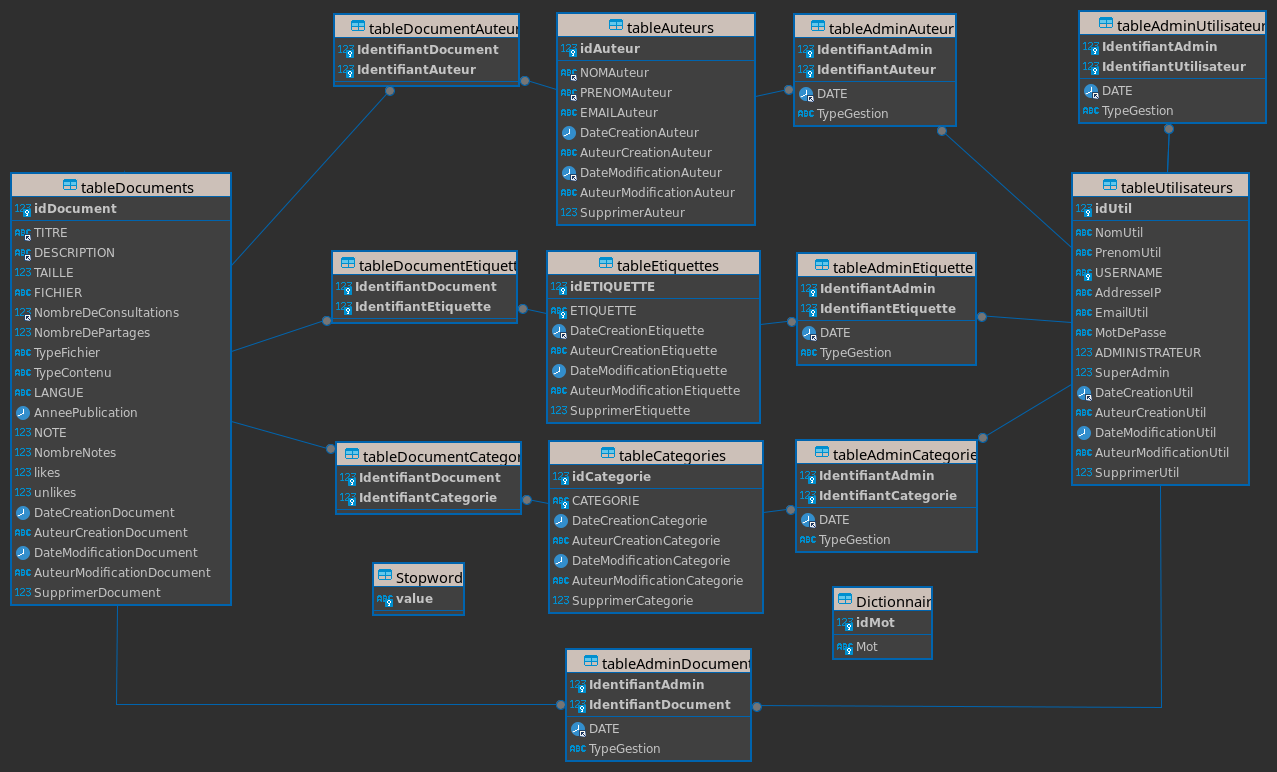
\includegraphics[width=0.8\textwidth]{Pictures/DiagrammeDeDonnees.png}
				\centering
				\caption{Sch\'ema des donn\'ees}
				\label{SchemaDeDonnees}
			\end{figure}